\documentclass{neu_handout}
\usepackage{url}
\usepackage{amssymb}
\usepackage{amsmath}
\usepackage{marvosym}
\usepackage{graphicx}
\usepackage[pdftex]{graphicx}
\usepackage{subfigure}
\graphicspath{ {images/} }
\everymath{\displaystyle}

% Professor/Course information
\title{Milestone 3 - UFOs}
\author{Abby, Emily, Lydia and Peter (The Conspiracists)}
\date{April 2018}
\course{CS 7295}{Information Visualization}

\begin{document}

\section*{1 Project Information}
1. GitHub Repository (URL): https://github.ccs.neu.edu/emilydutile/info-viz-ufos \\

*For information on building and running locally to see the current visualization, please see the README.md file in the repository. Running 'npm start' will automatically launch a localhost on your machine to view the application. For hosting the web app, Heroku\footnote{\url{https://www.heroku.com/}} will be set up and used for user viewing/demos.\\\\


2. Final report can be viewing on Google Drive\footnote{\url{https://drive.google.com/drive/u/1/folders/1uudnVKkbhPkOedPmMVpuFCdeWP3en1S0}} or on GitHub \footnote{\url{https://github.ccs.neu.edu/emilydutile/info-viz-ufos/tree/master/report/final}} \\\\


3. Current state of the visualization:\\
\begin{figure}[h]
\centering
{
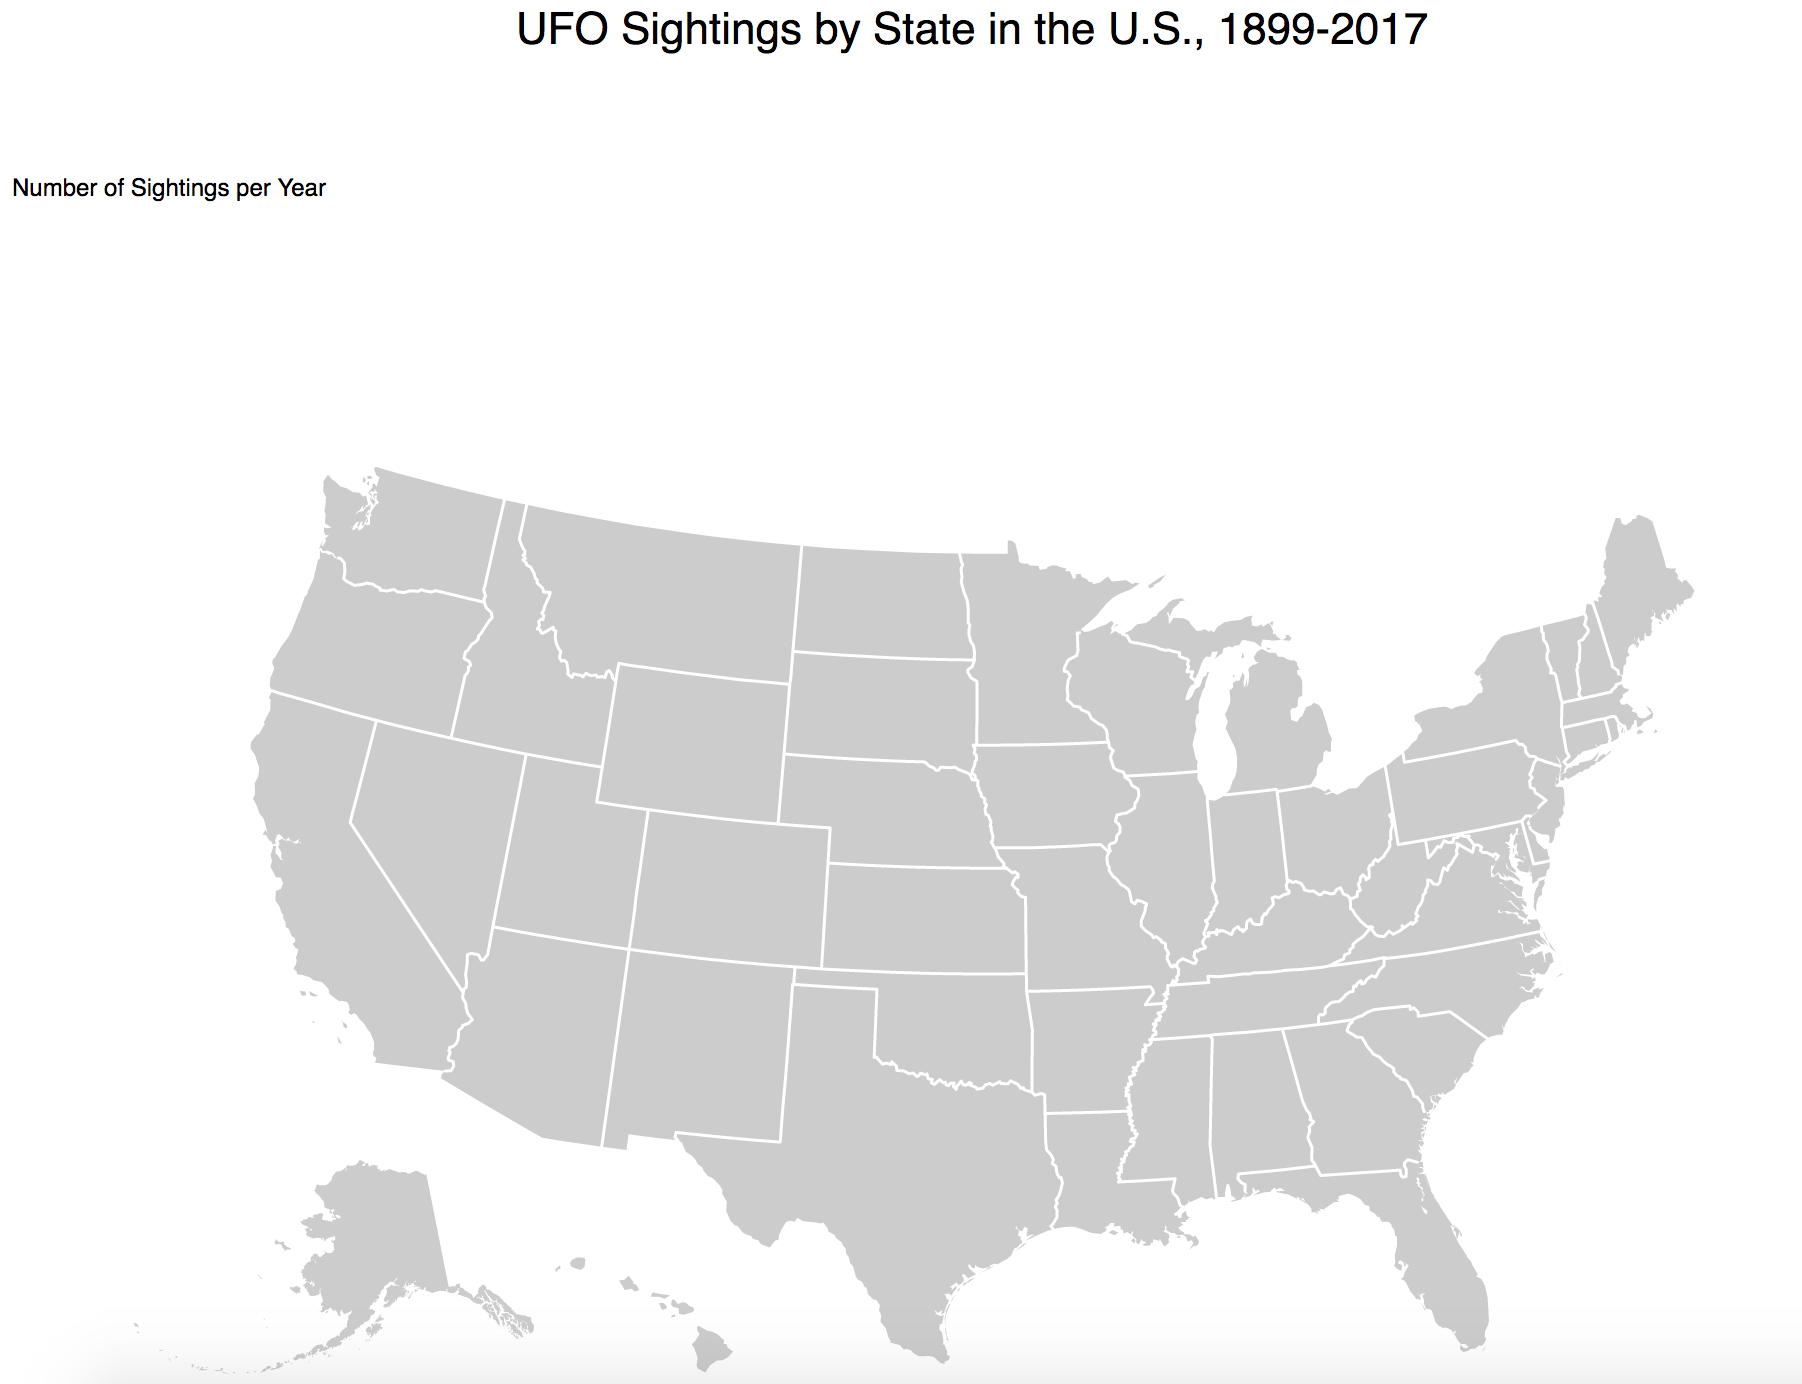
\includegraphics[width=0.6\linewidth]{site}
}
\end{figure}


4. Changes/additional details\\

After working with the d3 geojson map, the zoom/transition function was not as smooth or easy to implement as we anticipated. Due do this, we made new sketches/wireframes that fit our task analysis along with project requirements. The site will be more like the MBTA site in class, having the user scroll down the page to view details and visualizations. Brushing and linking between the time series bar chart and the chloropleth map will be available. This will give users an overall details view along with a specific period of time if selected. For more specific details by state (as seen before), users can select a state from a drop down in order to see individual sighting information per state.

\begin{figure}[h]
\centering
{
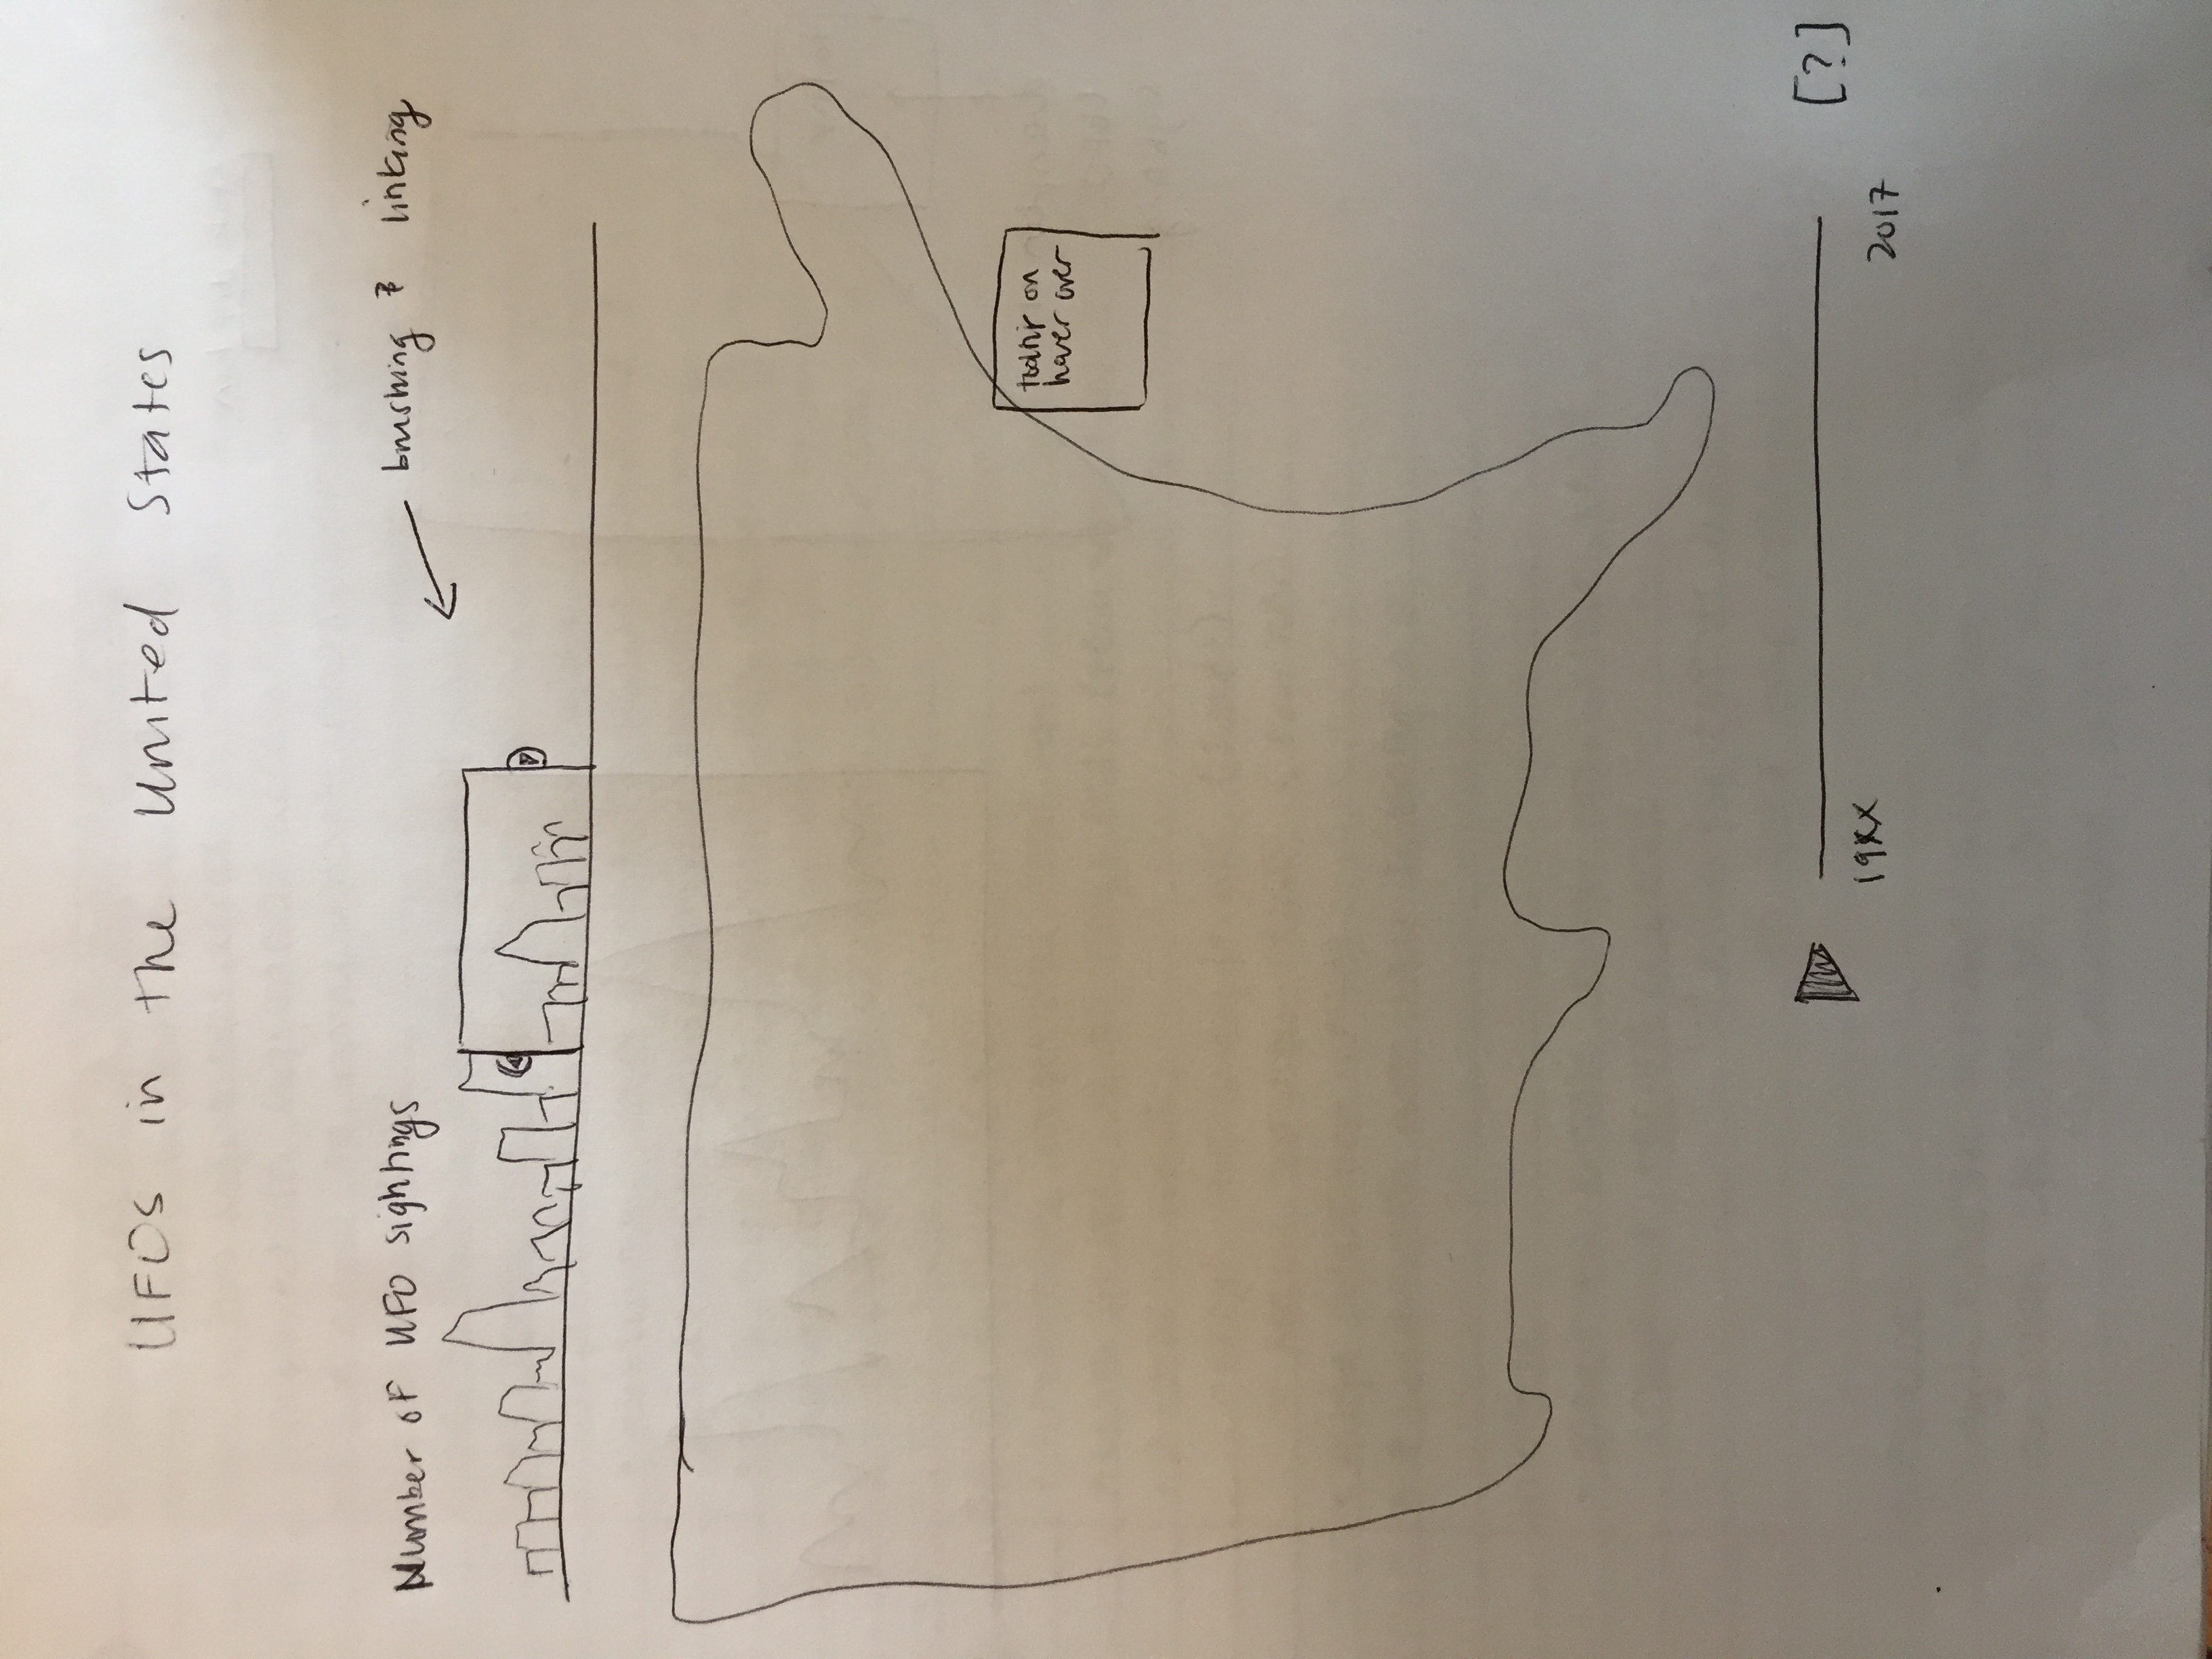
\includegraphics[width=0.8\linewidth]{image1}
}
\end{figure}

\begin{figure}[h]
\centering
{
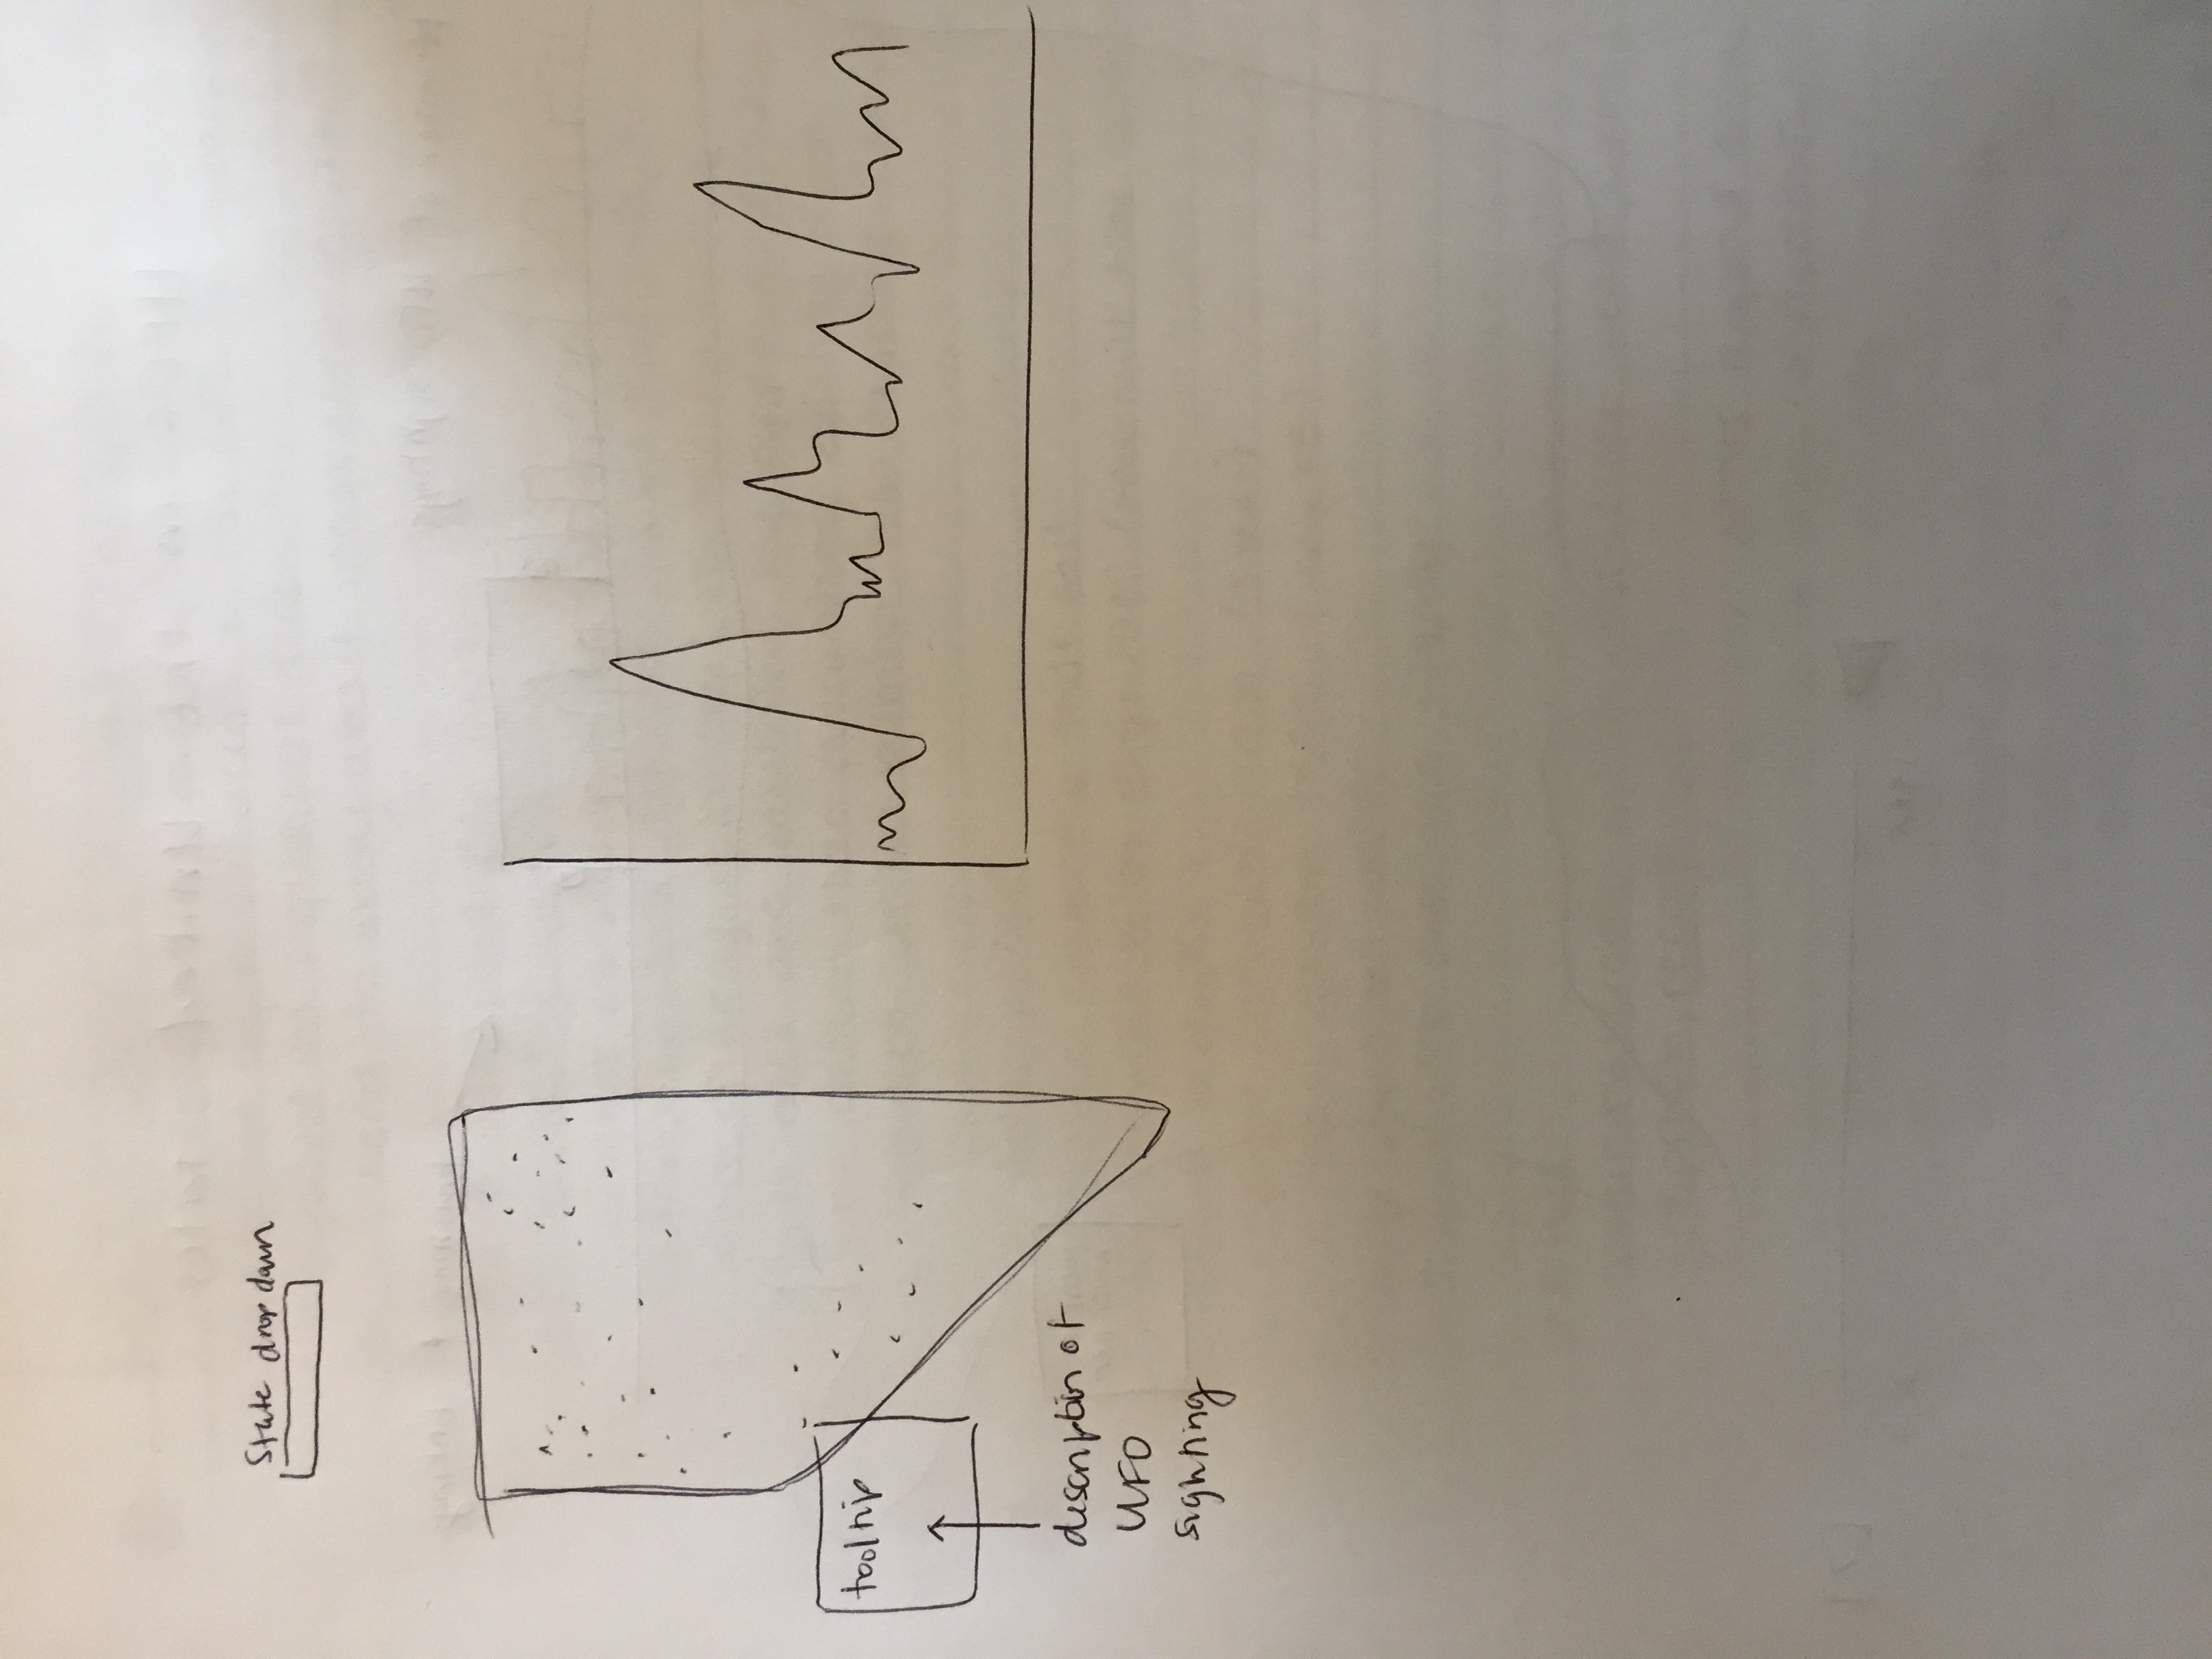
\includegraphics[width=0.8\linewidth]{image2}
}
\end{figure}


\end{document}
